\documentclass{letnab}
\pagestyle{fancy}
\usepackage{tabu}
\usepackage{units}
\usepackage{lscape}
\usepackage{ctable} % for \specialrule command

\usepackage{booktabs}
\rhead{Общая физика МФТИ}
\lhead{Лабораторная работа 2.4.1} 

\renewcommand{\headrulewidth}{2pt}
\begin{document}

	\begin{titlepage}
		
		
		
		\center % Center everything on the page
		
		
		
		%----------------------------------------------------------------------------------------
		%	HEADING SECTIONS
		%----------------------------------------------------------------------------------------
		
		\textsc{\LARGE Московский Физико-Технический Институт}\\[1,5cm] % Name of your university/college
		% Major heading such as course name
		\textsc{\Large Кафедра общей физики}\\[0.5cm]
		\textsc{\large Отчет о выполнении лабораторной работы \textnumero  2.1.1}\\[0.5cm] % Minor heading such as course title
		
		%----------------------------------------------------------------------------------------
		%	TITLE SECTION
		%----------------------------------------------------------------------------------------
		
		\HRule
		\\[0.4cm]
		{ \huge \bfseries Измерение удельной теплоёмкости воздуха при постоянном давлении}
		\\[0.2cm] % Title of your document
		\HRule
		\\[1.5cm]
		
		
		
		%----------------------------------------------------------------------------------------
		%	AUTHOR SECTION
		%----------------------------------------------------------------------------------------
		
		\begin{minipage}{0.7\textwidth}
			\begin{center} \large
				\emph{Автор:} Алексей \textsf{Домрачев} 615 группа
			\end{center}
		\end{minipage}
		\\[1.0cm]
		\begin{minipage}{0.9\textwidth}
			\begin{center} \large
				\emph{Преподаватель:} Александр Дмитриевич \textsf{Калашников} % Supervisor's Name
			\end{center}
		\end{minipage}
		\vfill 
	%	\begin{bottompar}
			
\includegraphics[width = 80 mm]{logo.png}	\\[1,0cm]
			{\large \today}
	%	\end{bottompar}
		% Fill the rest of the page with whitespace
		
	\end{titlepage}



\paragraph{Цель работы:}
исследование зависимости $P(T)$ давления насыщенного пара от температуры
и определение молярной теплоты парообразования~$L$
с использованием уравнения Клапейрона\,--\,Клаузиуса.
\paragraph{В работе используются:}термостат; герметический сосуд, заполненный исследуемой жидкостью; отсчетный микроскоп.
\paragraph{Устройство установки}.\\
\begin{minipage}{90mm}
	\begin{figure}[H]
	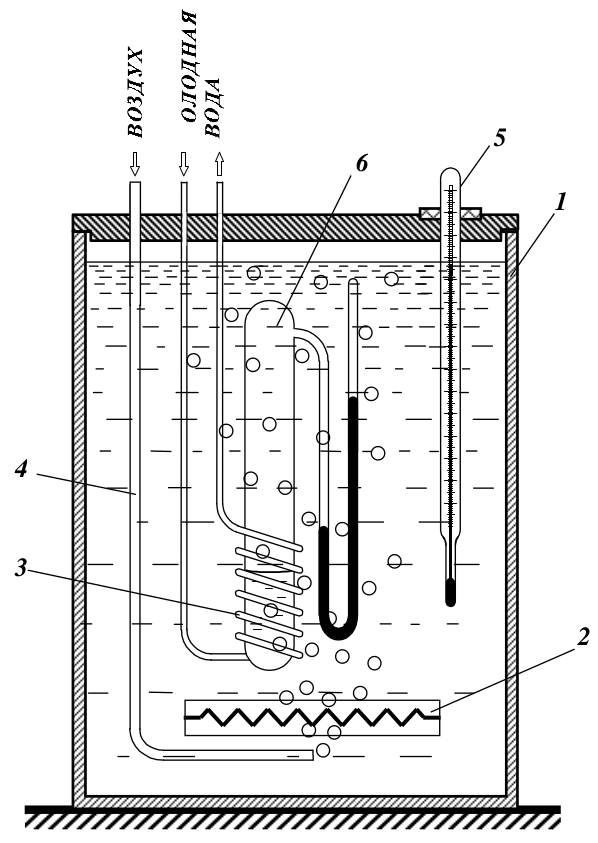
\includegraphics[width = 80mm]{station.png}
	\caption{Экспериментальная установка}
	\end{figure}
\end{minipage}
\begin{minipage}{90 mm}
	Заполненная водой ёмкость подключена к термостату. В неё погружена запаянная ёмкость с исследуемой жидкостью(вода); над жидкостью находится только её насыщенный пар, давление которого определяется по манометру при помощи отсчётного микроскопа. Таким образом можно исследовать зависимость давления насыщенного
	пара исследуемой жидкости от температуры $P(T)$, а затем определить $L$.\\[0.4cm]
	Необходимо выдерживать скорость изменения температуры не слишком большой, поскольку в противном случае не будет успевать устанавливаться равновесие между теплообменной и исследуемой жидкостью, а также между исследуемой жидкостью и её парами. В целях контроля данные измерения производятся как при нагревании, так и при охлаждении жидкости. 
\end{minipage}
\paragraph{Теория.}
Формула Клапейрона\,--\,Клаузиуса:\; $\dfrac{dP}{dT}=\dfrac{L}{T(V_2-V_1)}$, где $L$ --- теплота испарения жидкости, $V_2$ --- молярный объем паров жидкости, $V_1$ --- молярный объем жидкости.
\begin{table}[H]
	\centering
	\caption{Данные из лабника}
	\begin{tabular}{|c|c|c|c|c|c|c|}
		\hline
		Вещество & $T_{\text{кип}}$, К & $V_1$, $10^{-6}\text{м}^3/моль$ & $V_2$, $10^{-3}\text{м}^3/\text{моль}$ & $b$, $10^{-6}\text{м}^3/\text{моль}$ & $a,\, \frac{{\text{Па}}\cdot\text{м}^6}{\text{моль}^2}$  & $a/V_2^2$, кПа \\ \hline
		Вода     & 373                      & 18                              & 31                              & 26                            & 0,4                                                                                               & 0,42           \\ \hline
	\end{tabular}
\end{table} 
Из таблицы видно, что молярный объём газовой фазы существенно
(на несколько порядков) больше объёма жидкой фазы, последним пренебрежём. Кроме того, будем считать, что насыщенный пар удовлетворяет уравнению состояния идеального газа, \\а L зависит от T слабо: 
\begin{equation*}
    \Delta V \cong \dfrac{RT}{P} \then \dfrac{dP}{dT} \cong \dfrac{LP}{RT^2} \then L \cong R \dfrac{dP}{P} \dfrac{T^2}{dT} \then \fbox{$L \cong -R \dfrac{d(\ln P)}{d(1/T)}$}
\end{equation*}



\paragraph{Ход работы}Измерим разность уровней в ртутном U-образном манометре с помощью микроскопа и температуру по
термометру: $h_0 = 26.1$ мм рт.ст., $T_0=299$ К.
Включим термостат. Плавно повысим температуру
до 41 в течение 90 минут, при этом через каждый
градус необходимо измерять давление и температуру.\\[-0.5cm]
\begin{table}[H]
	\centering
	\caption{Данные при повышении температуры}
	\begin{tabular}{|c|c|c|c|c|c|c|c|}
		\hline
		$T$, К & $P_\text{верх}$, торр & $P_\text{низ}$, торр & $P$, торр & $P$, КПа & $t$, $C^\circ$ & $10^3\cdot1/T$ & $\ln P$ \\ \specialrule{.2em}{.1em}{.1em} 
		\multicolumn{8}{|c|}{данные при повышении температуры} \\ \hline
		301    & 57,6                     & 29,5                 & 28,1      & 3,75     & 28             & 3,32           & 1,32    \\ \hline
		302    & 57,3                     & 28                   & 29,3      & 3,91     & 29             & 3,31           & 1,36    \\ \hline
		303    & 58,7                     & 27,2                 & 31,5      & 4,20     & 30             & 3,30           & 1,43    \\ \hline
		304    & 59,9                     & 26,9                 & 33        & 4,40     & 31             & 3,29           & 1,48    \\ \hline
		305    & 60,3                     & 21,7                 & 38,6      & 5,15     & 32             & 3,28           & 1,64    \\ \hline
		306    & 61,9                     & 24,4                 & 37,5      & 5,00     & 33             & 3,27           & 1,61    \\ \hline
		307    & 67,2                     & 28,2                 & 39        & 5,20     & 34             & 3,26           & 1,65    \\ \hline
		308    & 64,5                     & 22,7                 & 41,8      & 5,57     & 35             & 3,25           & 1,72    \\ \hline
		309    & 64,3                     & 20                   & 44,3      & 5,91     & 36             & 3,24           & 1,78    \\ \hline
		310    & 66,1                     & 20,8                 & 45,3      & 6,04     & 37             & 3,23           & 1,80    \\ \hline
		311    & 68,4                     & 18                   & 50,4      & 6,72     & 38             & 3,22           & 1,90    \\ \hline
		312    & 63,6                     & 12,2                 & 51,4      & 6,85     & 39             & 3,21           & 1,92    \\ \specialrule{.2em}{.1em}{.1em}
		\multicolumn{8}{|c|}{данные при понижении температуры} \\ \hline
		311  & 69,6    & 17,9   & 51,7          & 6,89  & 40    & 3,22     & 1,93 \\ \hline
		310  & 61,5    & 18,5   & 43            & 5,73  & 37    & 3,23     & 1,75 \\ \hline
		309  & 65,3    & 19,5   & 45,8          & 6,11  & 35    & 3,24     & 1,81 \\ \hline
		307  & 64,6    & 21,8   & 42,8          & 5,71  & 33    & 3,26     & 1,74 \\ \hline
		306  & 61,7    & 22,3   & 39,4          & 5,25  & 31    & 3,27     & 1,66 \\ \hline
		305  & 61,1    & 24     & 37,1          & 4,95  & 29    & 3,28     & 1,60 \\ \hline
		304  & 60,3    & 24,8   & 35,5          & 4,73  & 27    & 3,29     & 1,55 \\ \hline
		303  & 59,9    & 25,3   & 34,6          & 4,61  & 25    & 3,30     & 1,53 \\ \hline
		302  & 58,1    & 26,9   & 31,2          & 4,16  & 23    & 3,31     & 1,43 \\ \hline
		301  & 57,3    & 27,3   & 30            & 4,00  & 21    & 3,32     & 1,39 \\ \hline
		300  & 57,8    & 27,6   & 30,2          & 4,03  & 22    & 3,33     & 1,39 \\ \hline
		299  & 56      & 28,5   & 27,5          & 3,67  & 23    & 3,34     & 1,30 \\ \hline
		298  & 55,8    & 30,8   & 25            & 3,33  & 24    & 3,36     & 1,20 \\ \hline
		297  & 54      & 30     & 24            & 3,20  & 25    & 3,37     & 1,16 \\ \hline
		296  & 54,4    & 29,5   & 24,9          & 3,32  & 26    & 3,38     & 1,20 \\ \hline
		295  & 53      & 32,8   & 20,2          & 2,69  & 27    & 3,39     & 0,99 \\ \hline
		294  & 53      & 31     & 22            & 2,93  & 28    & 3,40     & 1,08 \\ \hline
	\end{tabular}
\end{table}
\newpage
\paragraph{Построим графики в координатах $1/T$, $\ln \Delta P.$}
Посчитав с помощью МНК коэффициент наклона получим $k$ при повышении температуры: $k = -5.2 \pm 0.2\cdot 10^3$, 1/К.
\begin{figure}[H]
	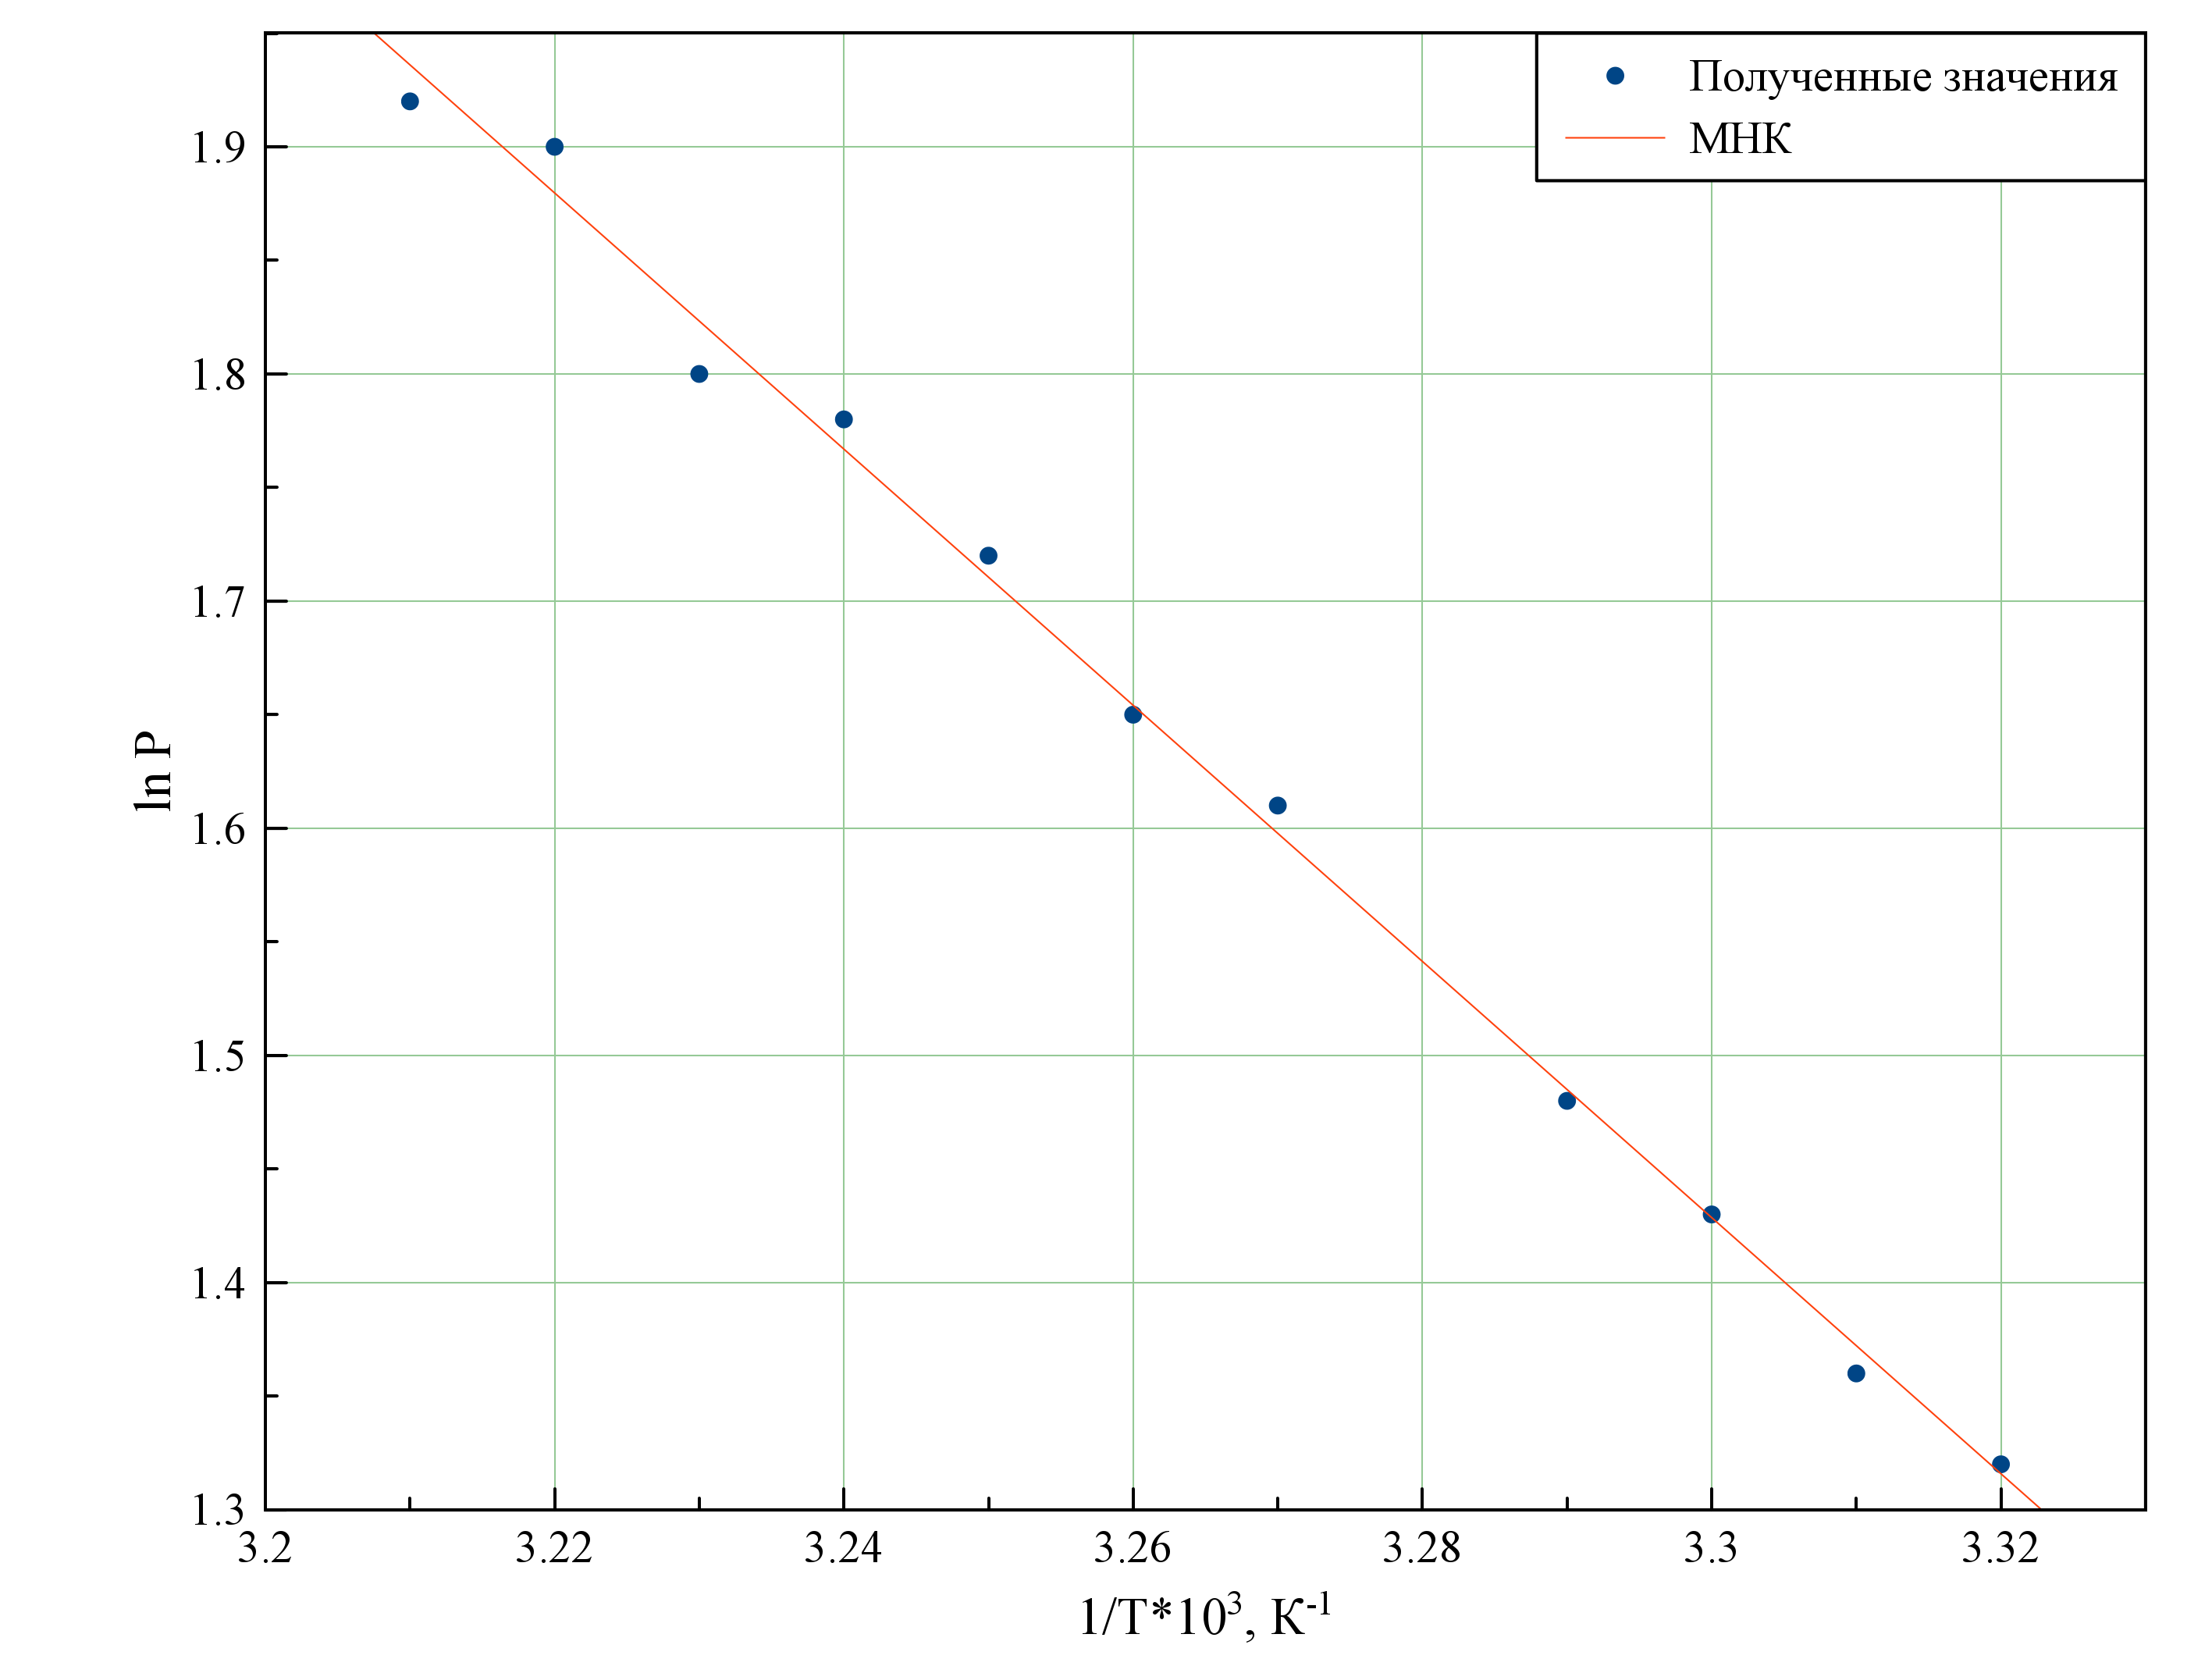
\includegraphics[width = 135mm]{graph1.png}
	\caption{При повышении температуры}
\end{figure}
Аналогично для понижения : $k = -5.0 \pm 0.1\cdot 10^3$, 1/К.
\begin{figure}[H]
	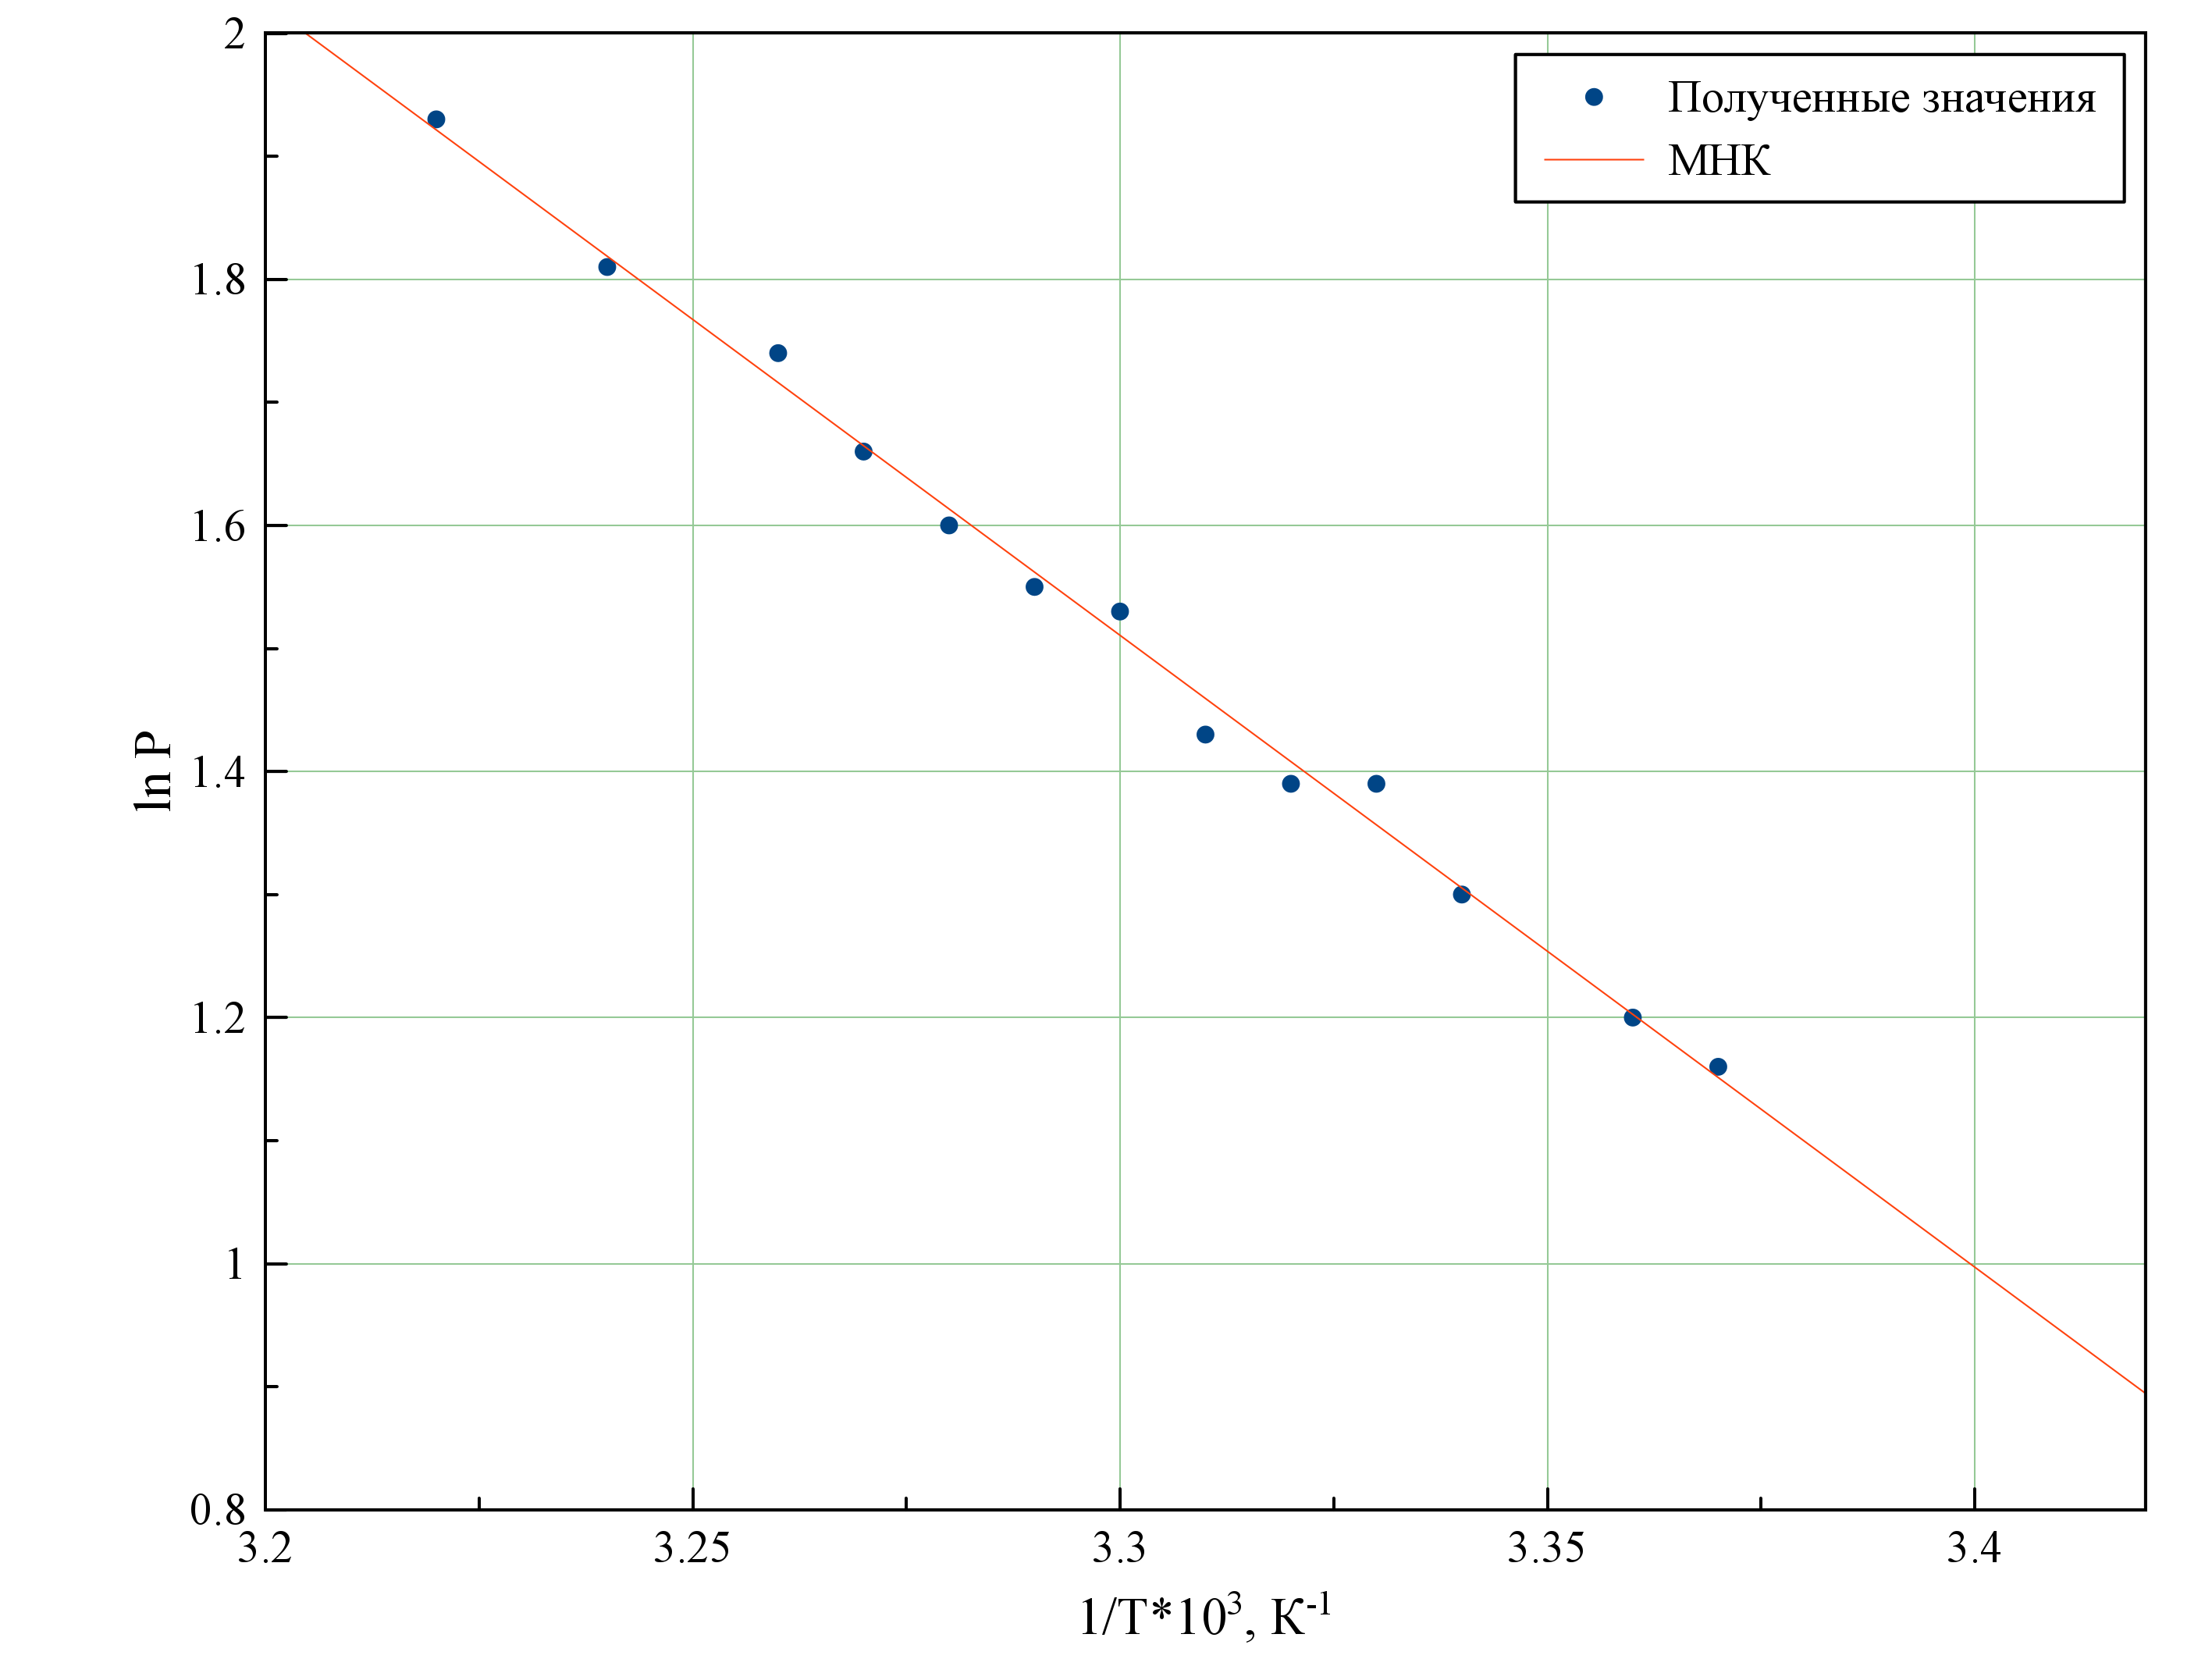
\includegraphics[width = 135mm]{graph2.png}
	\caption{При понижении температуры}
\end{figure}

Итак $L = -R \cdot k$\\
$L_1 = 43.2$ кДж/моль, $\sigma_{L_1} = 1.7$ кДж/моль.\\
$L_2 = 41.6$ кДж/моль, $\sigma_{L_2} = 1.3$ кДж/моль.\\
Значения~$L$, вычисленные по данным, полученным при нагревании и охлаждении,
совпадают в пределах погрешности , поэтому применим МНК на всей выборке.\\
\Large В итоге получим \fbox{$L = 40.0 \pm 1.4$, кДж/моль} \normalsize 
\paragraph{Вывод}Значения $L_1$ и $L_2$ близки друг к другу в пределах погрешности. Табличное значение среднего L --- 41 кДж/моль [himikatus.ru/art/ch-act/0220.php], что так же верно в пределах погрешности. График на понижении температур позволяет вычислить L с наибольшей точностью.
\end{document}
